\newpage
\section{О двудольных графах}

Наравне с деревьями, очень распространены двудольные графы.
	
\mysubsection{Базовые понятия двудольных графов}	
	
\begin{definition}
	\emph{Двудольный граф}~---~граф, вершины которого можно разбить на два непересекающихся множества так, что никакое ребро графа не соединяет вершины одного множества. Обозначается $G[X, Y]$, где $X$ и $Y$~---~две доли графа.
\end{definition}

	Заметим, что как таковых двудольных полных графов нет при $|V| \geqslant 2$, однако понятие полноты обоществляется на двудольный граф следующим образом.
	
\begin{definition}
	Граф $G$ называется \emph{полным двудольным}, если он является двудольным графом $G[X, Y]$ и для произвольных $x \in X$ и $y \in Y$ ребро $(x, y) \in E$.
\end{definition}

	Для <<полных>> двудольных графов принято обозначение~---~$K_{n,m}$, где $n$ и $m$~---~число вершин в каждой доле графа.

\begin{statement}
	В полном двудольном графе $K_{n, m}$ ровно $n\cdot m$ рёбер.
	
	\emph{Доказательство.} Вспомним, что любое ребро двудольного графа соединяеет вершины из разных долей. Значит, чтобы получить общее число рёбер надо перемножить число способов выбрать из первой доли одну вершину на число способов выбрать вершину из второй доли. Следовательно, общее число рёбер равно $C_n^1 \cdot C_m^1 = nm$. ч.т.д.
\end{statement}
	
\begin{example}
	На танцы пришли $n$ девушек и $n$ юношей. Каждый юноша знаком с двумя девушками, а каждая девушка знакома с двумя юношами. Докажите, что собравшихся можно разбить на $n$ смешанных пар так, чтобы в каждой паре юноша и девушка были знакомы.
	
	\emph{Решение.} Обозначим через вершины графа~---~юношей и девушек, а ребрами соединим тех, кто знаком. Тогда весь граф будет состоять из четных циклов. А каждый четный цикл можно, очевидно, разбить на пары вершин, которые будут соединены ребром.
\end{example}

\begin{paracol}{2}
	Совершенно неожиданно оказывается, что некоторые графы являются двудольными, хотя, увидев их, читатель вряд ли бы моментально согласился с этим.

\begin{definition}
	Граф $K_{n, 1}$ называется \emph{звездой}.
\end{definition}
\begin{definition}
	\emph{Граф-цикл}~---~связный граф, в котором у каждой вершины степень равна двум. Обозначается так $С_n$.
\end{definition}

\switchcolumn
 
\begin{center}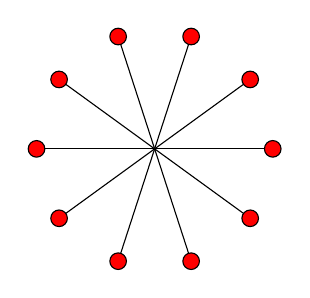
\begin{tikzpicture}
	\tikzstyle{every node}=[circle, draw, fill=red, inner sep=0pt, minimum width=6pt]
	\foreach \x in {0,36,...,324}
    {
    	
    	\draw (\x:1.5) -- (0, 0);
    	\draw (\x:1.5) node {};
    };
\end{tikzpicture}

	\small Рис. N. Звезда $K_{10, 1}$
\end{center}\end{paracol}

	При любом $n$ звезда будет двудольным графом и при чётных $n$ граф-цикл $C_n$ будет двудольным (см. рис. N).

\mysubsection{Паросочетание. Лемма Холла}

	Центральное понятие, связанное с двудольными графами,~---~это паросочетание.
	
\begin{definition}
	\emph{Паросочетание или независимое множество рёбер}~---~это набор попарно несмежных рёбер. \emph{Совершенным паросочетанием} называется такое паросочетание, что любая вершина смежна одному из его рёбер. 
\end{definition}

\begin{theorem}[Холла]
	Если в двудольном графе $G[X, Y]$ для любого набора вершин $x_1, x_2, \dots, x_k \in X$ есть не менее $k$ вершин в доле $Y$, которые смежны с одной из вершин $x_i$, то существует подмножество вершин $Y' \subset Y$ такое, что в $G[X, Y']$ есть совершенное паросочетание.
	
	\emph{Альтернативное условие.} Есть $n$ юношей и несколько девушек. Известно, что для любых $k$ юношей число знакомых им в совокупности девушек не меньше $k$. Тогда все юноши могут выбрать по невесте из числа своих знакомых.
	
	\emph{Доказательство.} Допустим противное, то есть что максимальное паросочетание не содержит всех юношей. Тогда рассмотрим юношу $C$ (от <<сыч>>), который не входит в это паросочетание.
	
	Он должен быть знаком хотя бы с одной девушкой. Если он знаком с девушкой не из паросочетания, то мы можем составить пару. Противоречие. Тогда он знаком с какой-то девушкой из паросочетания. Обозначим эту девушку за $Д_1$, а её юношу~---~$Ю_1$. Следовательно, по условию теоремы для юношей $Ю_1$ и $C$ есть две девушки, с которыми они знакомы. Такими рассуждениями, приходим к тому, что $Ю_1$ должен быть знаком с $Д_2$, $Ю_2$ должен быть знаком с $Д_3$... В конце будет обязательно $Ю_k$, который будет знаком с девушкой не из паросочетания. Тогда переженим их и число пар увеличится на 1. Противоречие. Следовательно, исходное максимальное паросочетание было искомым. ч.т.д. 
\end{theorem}

	Иначе эта теорема называется теоремой о сватовстве или свадьбах. Несмотря на видимую сложность, эта теорема имеет необыкновенно широкое в задачах, с виду не похожих на задачу на графы.
	
\begin{example}
	Из шахматной доски $8 \times 8$ вырезали семь клеток. Докажите, что на оставшуюся доску можно поставить $8$ ладей так, чтобы они не били друг друга.
	
	\emph{Решение.} Рассмотрим двудольный граф $G[X, Y]$, где в доле $X$ будут вершинами строки, а в доле $Y$~---~столбцы, а соединены будут те, на пересечение которых есть невырезанная клетка. Заметим, что условие Холла выполняется. Следовательно, есть совершенное паросочетание, то есть мы можем разбить строки и столбцы на $8$ непересекающихся множества так, что их пересечение будет невырезанной клеткой. На эти клетки и поставим ладей. ч.т.д.
\end{example}

\newpage
\mysubsection{Задачи}
	
\begin{exersize}
	В классе $15$ мальчиков. Известно, что каждый из них знаком с ровно тремя девочками, а каждая девочка знакома ровно с пятью мальчиками. Сколько в классе детей?
\end{exersize}

\begin{exersize}
	Докажите, что любое дерево является двудольным графом.
\end{exersize}

\begin{exersize}(Канель-Белов А.Я., Ковальджи А.К. Как решают нестандартные задачи)
	На математической олимпиаде было предложено $20$ задач. На закрытие пришло $20$ школьников. Каждый из них решил по две задачи, причем выяснилось, что среди пришедших каждую задачу решило ровно два школьника. Докажите, что можно так организовать разбор задач, чтобы каждый школьник рассказал одну из решенных им задач, и все задачи были разобраны.
\end{exersize}

\begin{exersize}(Канель-Белов А.Я., Ковальджи А.К. Как решают нестандартные задачи)
	В квадратной таблице $N \times N$ записаны неотрицательные числа так, что сумма в любой строке и в любом столбце равна $1$. Докажите, что в этой таблице можно выбрать $N$ положительных чисел, никакие два из которых не будут находиться в одной строке или столбце.
\end{exersize}

\begin{exersize}
	Определите при каких $m$ и $n$ полный двудольный граф $K_{m, n}$ будет эйлеровым. А при каких значениях он будет полуэйлеровым?
\end{exersize}

\begin{exersize}
	Докажите, что граф $Q_k$ является $k$-регулярным двудольным графом. Подсчитайте количество вершин и рёбер в таком графе.
\end{exersize}

\begin{exersize}[Бабичева Т.С., Бабичев С.Л., Жогов А. А., Яковлев И.В. <<Пособие по олимпиадной математике. Уровень А1>>]
	В графе каждая вершина~---~синяя или зеленая. При этом каждая синяя вершина связана с пятью синими и десятью зелеными, а каждая зеленая~---~с девятью синими и шестью зелеными. Каких вершин больше~---~синих или зеленых?	
\end{exersize}

\begin{exersize}[Агаханов Н.Х., Богданов И.И., Кожевников П.А., Подлипский О.К., Терешин Д.А. <<Всероссийские олимпиады школьников по математике 1993~---~2009: Заключительные этапы>>]
	В классе учится $15$ мальчиков и $15$ девочек. В день $8$ марта некоторые мальчики позвонили некоторым девочкам и поздравили их с праздником (никакой мальчик не звонил одной и той же девочке дважды). Оказалось, что детей можно единственным образом разбить на $15$ пар так, чтобы в каждой паре оказались мальчик с девочкой, которой он звонил. Какое наибольшее число звонков могло быть сделано?
\end{exersize}	  


\begin{exersize}[Агаханов Н.Х., Богданов И.И., Кожевников П.А., Подлипский О.К., Терешин Д.А. <<Всероссийские олимпиады школьников по математике 1993~---~2009: Заключительные этапы>>]
	$25$ мальчиков и несколько девочек собрались на вечеринке и обнаружили забавную закономерность. Если выбрать любую группу не меньше чем из $10$ мальчиков, а потом добавить к ним всех девочек, знакомых хотя бы с одним из этих мальчиков, то в получившейся группе число мальчиков окажется на $1$ меньше, чем число девочек. Докажите, что некоторая девочка знакома не менее чем с $16$ мальчиками.
\end{exersize}	 

\begin{exersize}[Агаханов Н.Х., Богданов И.И., Кожевников П.А., Подлипский О.К., Терешин Д.А. <<Всероссийские олимпиады школьников по математике 1993~---~2009: Заключительные этапы>>]
	В некоторой группе из $12$ человек сред каждых $9$ найдутся $5$ попарно знакомых. Докажите, что в этой группе найдутся $6$ попарно знакомых.
\end{exersize}	 

\begin{exersize}[Агаханов Н.Х., Богданов И.И., Кожевников П.А., Подлипский О.К., Терешин Д.А. <<Всероссийские олимпиады школьников по математике 1993~---~2009: Заключительные этапы>>]
	В лагерь приехало несколько пионеров, каждый из них имеет от $50$ до $100$ знакомых среди остальных. Докажите, что пионерам можно выдать пилотки, покрашенные в $1331$ цвет так, чтобы у знакомых каждого пионера были пилотки хотя бы $20$ различных цветов.
\end{exersize}	 